This is a software based workaround for our lab's computers to keep the in the
wired network. To implement the solution, following software is required to be
installed;

\begin{itemize}
 \item \textbf{Chrome} web browser
 \item \textbf{Anaconda} or another Pyhton distribution. 
 \item \textbf{Selenium} libraries for Anaconda to be able to interface with Selenium.
 \item \textbf{Selenium} Web Driver
\end{itemize}

\subsection{Preparation and Software Installations}
\subsubsection{Chrome Installation}
To install Chrome, go to following web page and download the suitable installer version
for your operating system (OS). \footnote{\url{https://www.google.com/chrome/}}

\subsubsection{Anaconda Installation}
To install Anaconda, go to web page and download Anaconda installer suitable for your  
OS. \footnote{\url{https://www.anaconda.com/products/individual}}. During the installation, at some
point installer will give you an option to add Anaconda to system path (\$PATH) as
shown in Figure\ref{fig:AnacondaInstall}.

\begin{figure}[H]
    \centering
	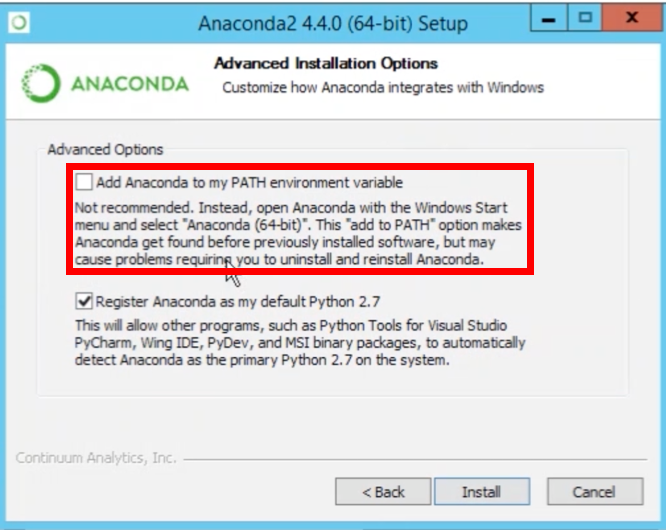
\includegraphics[angle=0,origin=c,width = .8\linewidth]{Section_Ethernet/Figures/Anaconda_PATH.png}
    \caption{Installation step for adding Anaconda to system path.}
    \label{fig:AnacondaInstall}
\end{figure}

Here, go ahead and click the box on the left to add Anaconda to system path. This will
make Anaconda your system-wide Python library. Its issues are not going to be discussed
here for simplicity.

\subsubsection{Selenium Library Installation}
To install Selenium libraries for allowing Anaconda to interface with Selenium web
driver you can use Anaconda Prompt as shown in Figure\ref{fig:AnacondaPrompt}.

\begin{figure}[H]
    \centering
    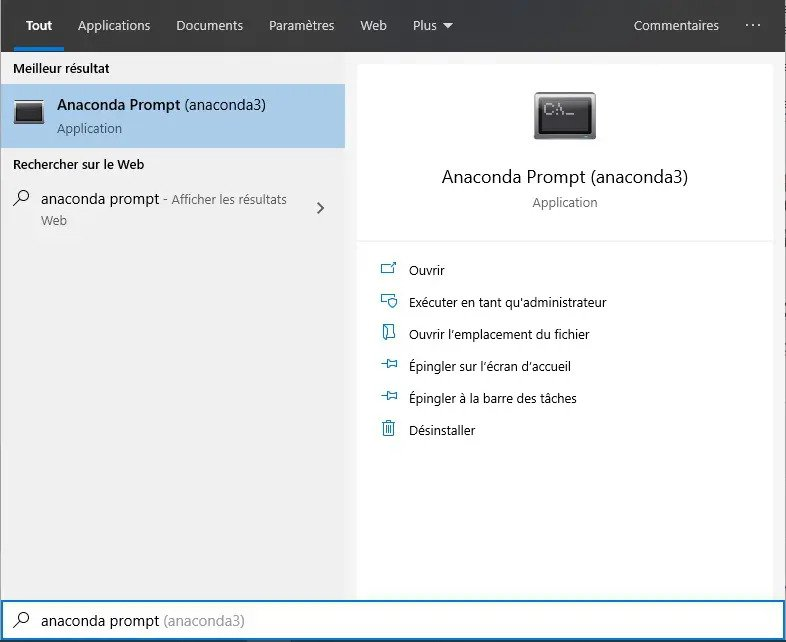
\includegraphics[angle=0,origin=c,width = .8\linewidth]{Section_Ethernet/Figures/anaconda-prompt.jpg}
    \caption{Opening up Anaconda Prompt.}
    \label{fig:AnacondaPrompt}
\end{figure}

In Anaconda Prompt, you can simply type \textbf{conda install -c conda-forge selenium}
and click \textbf{Enter}, as shown in Figure\ref{fig:SeleniumAnaconda}.

\begin{figure}[H]
    \centering
    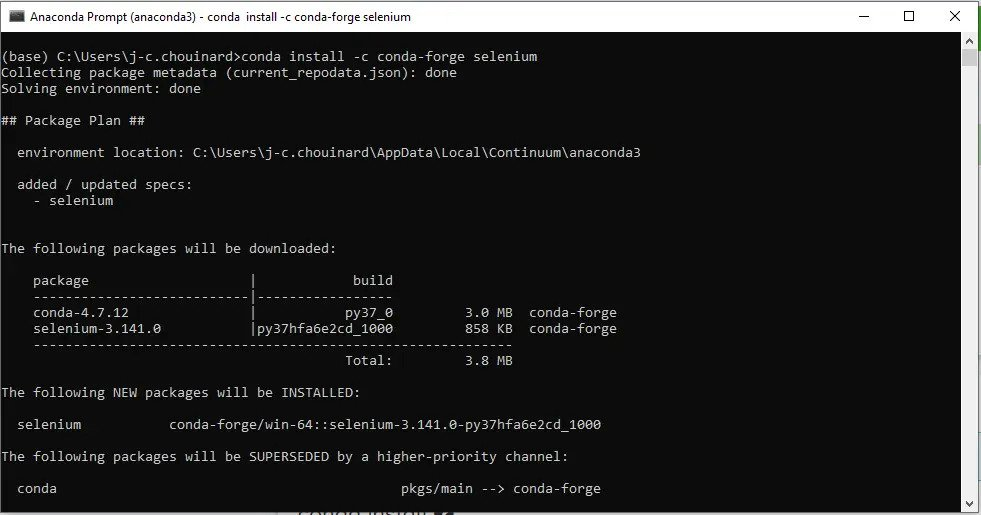
\includegraphics[angle=0,origin=c,width = .8\linewidth]{Section_Ethernet/Figures/install-selenium.jpg}
    \caption{Selenium library installation for Anaconda.}
    \label{fig:SeleniumAnaconda}
\end{figure}

Once Anaconda figures out where Selenium library is and possible additional required
libraries, it will ask your confirmation as shown in Figure
\ref{fig:SeleniumAnacondaConfirm}. Here you can type \textbf{y} and click \textbf{Enter}.

\begin{figure}[H]
    \centering
    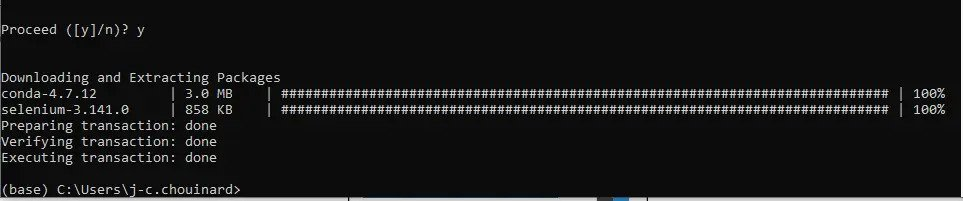
\includegraphics[angle=0,origin=c,width = .8\linewidth]{Section_Ethernet/Figures/confirm-screen.jpg}
    \caption{Selenium library installation confirmation screen.}
    \label{fig:SeleniumAnacondaConfirm}
\end{figure}

\subsubsection{Selenium WebDriver Installation}
To install Selenium WebDriver for allowing Selenium-Anaconda library to control the
web browser (\textbf{here we use Chrome!!!}), go to the following web page, 
\url{https://sites.google.com/a/chromium.org/chromedriver/} as shown in Figure
\ref{fig:WebDriverDownload}. 
\begin{figure}[H]
    \centering
    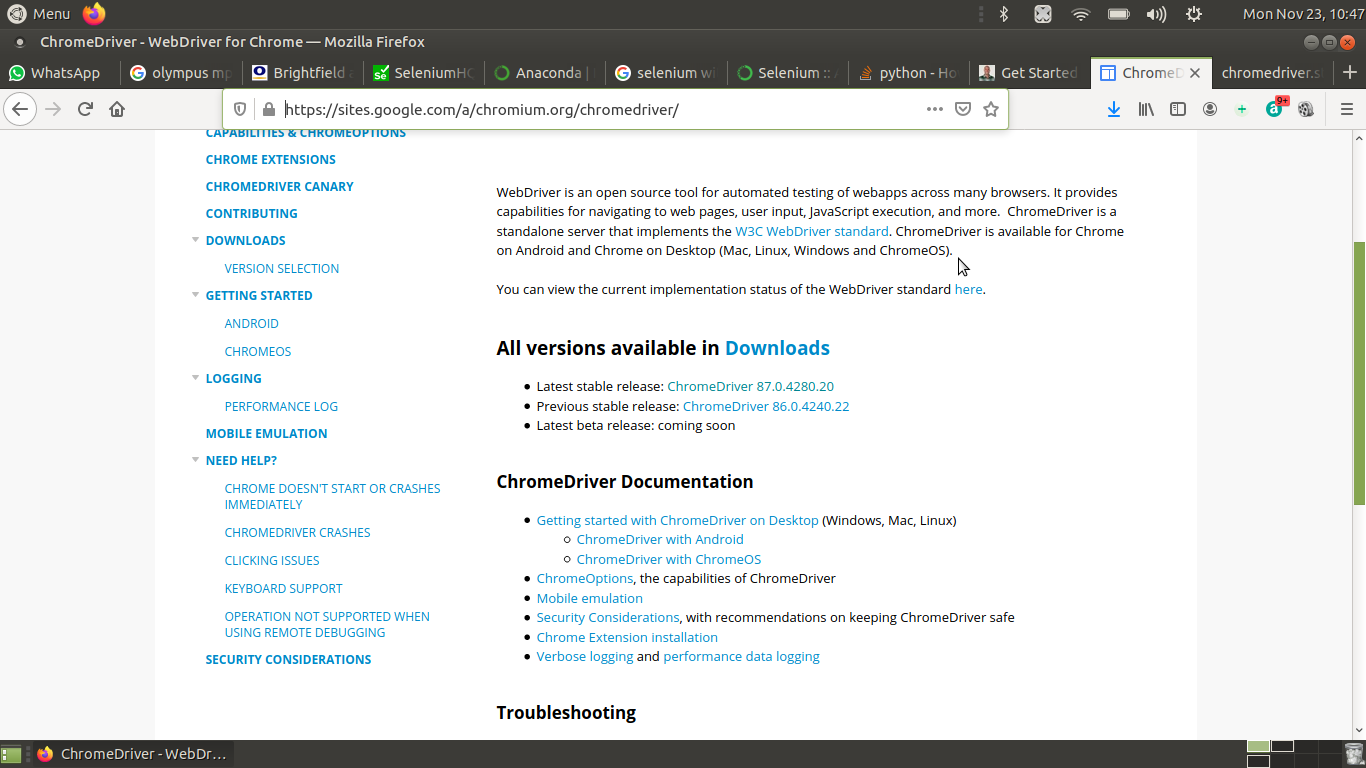
\includegraphics[angle=0,origin=c,width = .8\linewidth]{Section_Ethernet/Figures/WebDriverDownload.png}
    \caption{Selenium library installation confirmation screen.}
    \label{fig:WebDriverDownload}
\end{figure}

Within other options, click on the \textbf{Latest Stable Release}. This will direct you 
another web page with multiple files you can download as shown in Figure
\ref{fig:SeleniumWebDriver}. \textbf{Here, you have to download 32-bit driver!!!}

\begin{figure}[H]
    \centering
    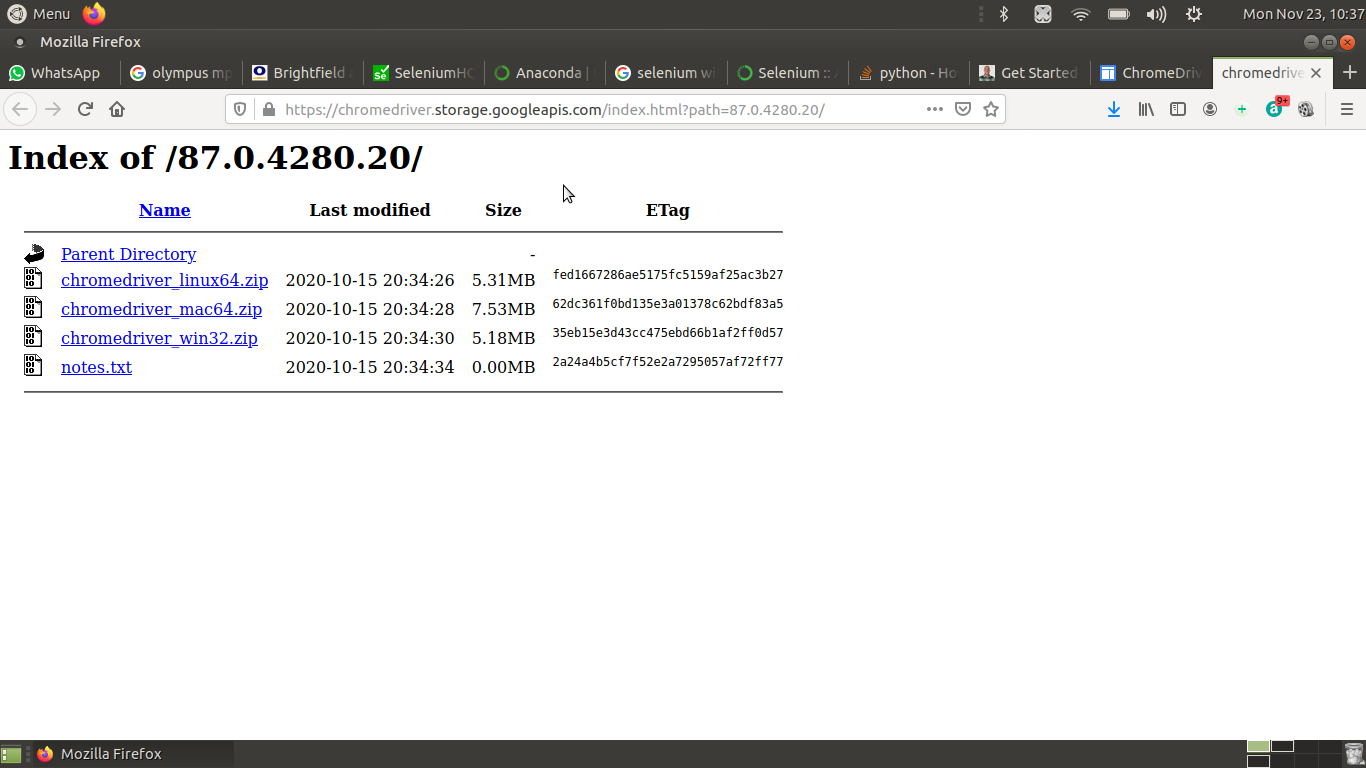
\includegraphics[angle=0,origin=c,width = .8\linewidth]{Section_Ethernet/Figures/PickWebDriver.png}
    \caption{Selenium library installation confirmation screen.}
    \label{fig:SeleniumWebDriver}
\end{figure}

Once download finishes, you can unzip the the webdriver file with any software you 
desire.

\subsection{Implementation-Coding}
To invoke Selenium I wrote Python Script. An overwiev of the code is as 
following;

\begin{enumerate}

 \item \textbf{Lines 1-4:} Imports essential libraries.
 \item \textbf{Lines 6-8:} Pings Google's DNS server to check whether the PC
        is connected to wired network. 
 \item \textbf{Lines 10-11:} If output of lines 6-8 are both indicating connection
        proceed to the end of the code.
 \item \textbf{Lines 12-27:} If PC is not connected;
 \textbf{Line 13:} Run Chrome driver
 \textbf{Line 14:} Send Chrome to university's Log-In page.
 Here "https://secure-access.morgan.edu/guest/ngnauth.php?" is a fixed string.
 "\&mac=f8:b1:56:b3:7a:0a\&\_browser=1" is the MAC address of our machine and
 browser number which is the default browser.
 \item \textbf{Lines 17-20:} Fill out the form on university's Log-In page
 using your username and password.
 \item \textbf{Lines 21-22:} Click the box to accept the terms.
 \item \textbf{Lines 23-24:} Click on the Accept button to Log-In.
 \item \textbf{Lines 25-27:} Wait for the webpage to load to university's homepage
 then close the browser.
 \item \textbf{Line 28:} Kill python.exe to stop the process cleanly.

\end{enumerate}


\begin{minted}[breaklines,mathescape,linenos]{python}
from selenium import webdriver
from selenium.webdriver.common.keys import Keys
import time
import os

temp = os.popen("ping 8.8.8.8").read()
test_connection1 = temp.find('PING: transmit failed. General failure.')
test_connection2 = temp.find('Request timed out.')

if (test_connection1 < 0 and test_connection2 < 0):
    print("Already connected. Exiting!!!")
else:
    driver = webdriver.Chrome()
    driver.get("https://secure-access.morgan.edu/guest/ngnauth.php?
                &mac=f8:b1:56:b3:7a:0a&_browser=1")
    
    elem1 = driver.find_element_by_id('ID_formcd662c6a_weblogin_user')
    elem1.send_keys("Peker.Milas")
    elem2 = driver.find_element_by_id('ID_formcd662c6a_weblogin_password')
    elem2.send_keys("Onder1981")
    elem3 = driver.find_element_by_id('ID_formcd662c6a_weblogin_visitor_accept_terms')
    elem3.click()
    elem4 = driver.find_element_by_id('ID_formcd662c6a_weblogin_submit')
    elem4.click()
    time.sleep(10)

    driver.close()
os.system("taskkill /F /im python.exe")
\end{minted}

\subsection{Implementation-Automatization}
As I have indicated above, the provided Python script is meant to execute once.
Therefore, to first sense a loss in wired connection and invoke the Selenium
for automatic Log-In, we use Windows' \textbf{Task Scheduler}. This is done as
following;

\begin{enumerate}
 
 \item Click on the Windows search bar and type Task Scheduler. This will pop
 a widow above Windows logo to let you run Task Scheduler which is shown in 
 Figure\ref{fig:TaskScheduler}
    \begin{figure}[H]
        \centering
        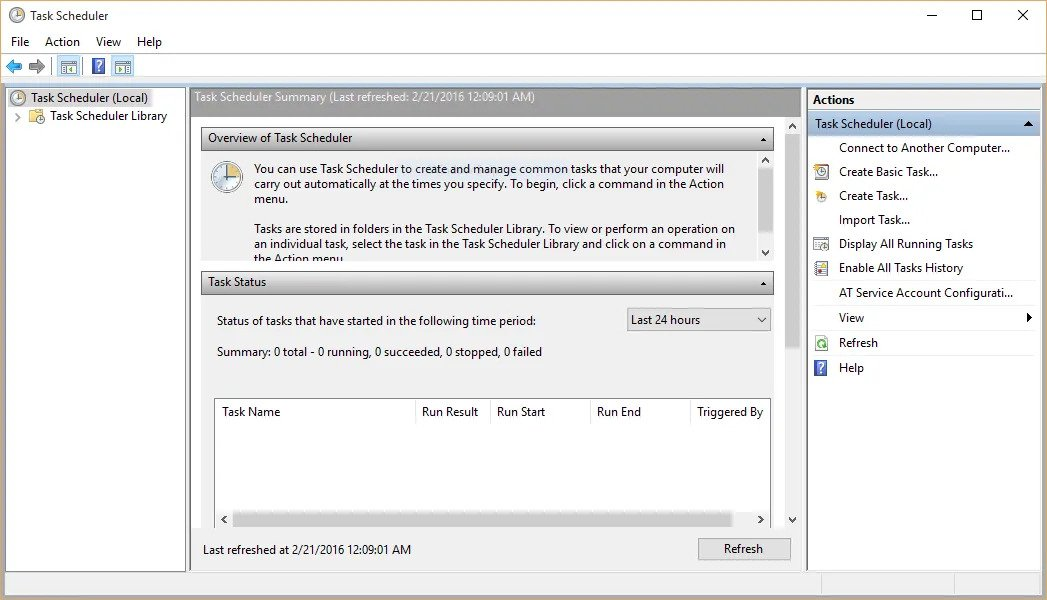
\includegraphics[angle=0,origin=c,width = .8\linewidth]{Section_Ethernet/Figures/Windows-10-Task-Scheduler.jpg}
        \caption{Windows10 Task Scheduler.}
        \label{fig:TaskScheduler}
    \end{figure}
 
 \item Click on the "Action$\rightarrow$Create Task", as shown in Figure
 \ref{fig:CreateTask}
    \begin{figure}[H]
        \centering
        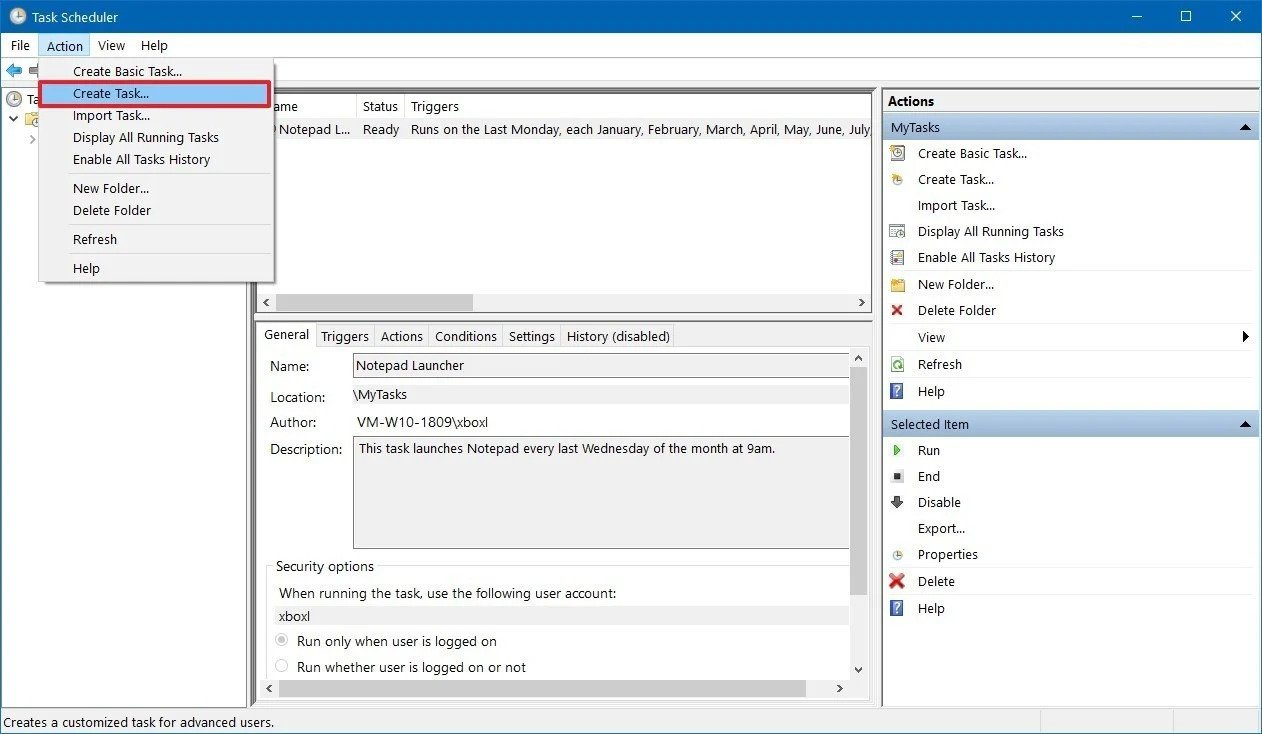
\includegraphics[angle=0,origin=c,width = .8\linewidth]{Section_Ethernet/Figures/create-task.jpg}
        \caption{Create a task in Task Scheduler.}
        \label{fig:CreateTask}
    \end{figure}
 
 \item In popped-up window, on General tab, as shown in Figure\ref{fig:TaskGeneral}, 
 give a unique name to your task and describe it for future reference.
 
    \begin{figure}[H]
        \centering
        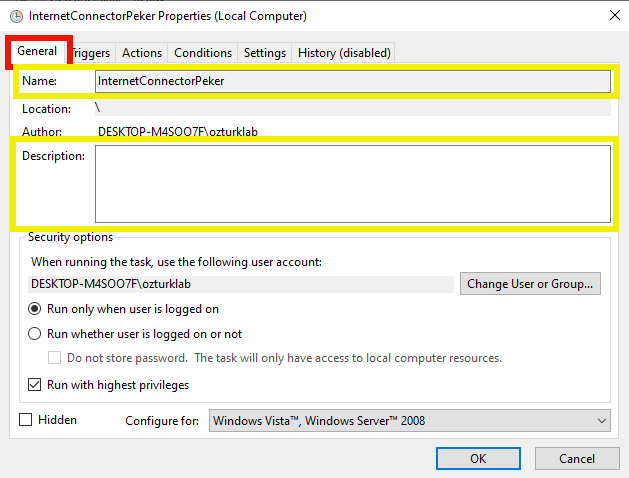
\includegraphics[angle=0,origin=c,width = .8\linewidth]{Section_Ethernet/Figures/TaskCreationName.png}
        \caption{Name and Description fields under General tab.}
        \label{fig:TaskGeneral}
    \end{figure}
    
 \item On the Triggers tab, as shown in Figure\ref{fig:TaskTriggers}, click on New.
 In popped-up window, set the Start time and date. Also make your task runs for One time. 
 Let the  task repeat at specified times (here every 30 minutes) and keep it run 
 indefinitely.
 
    \begin{figure}[H]
		\centering
		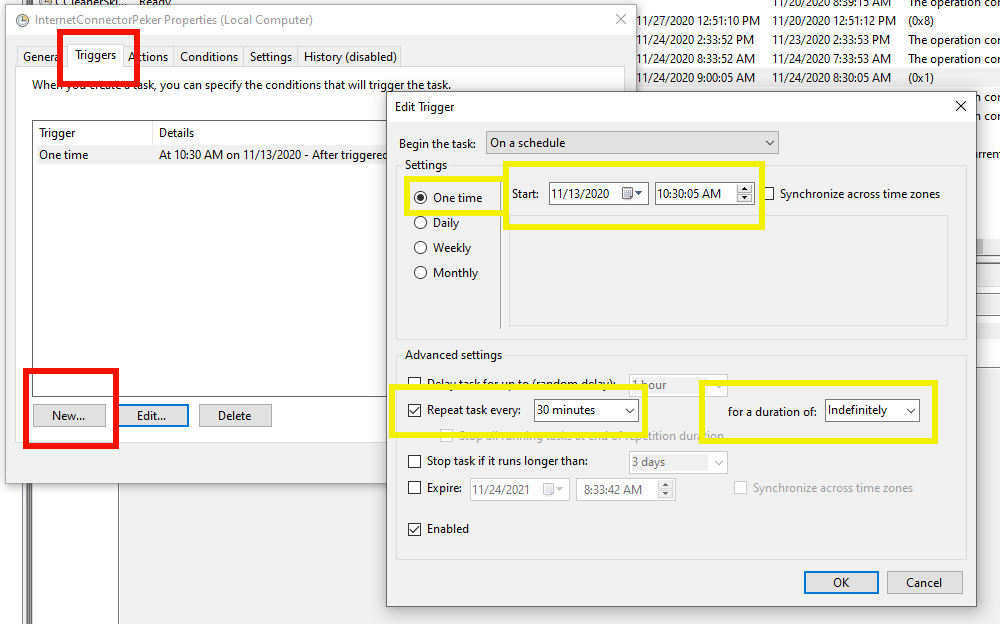
\includegraphics[angle=0,origin=c,width = .8\linewidth]{Section_Ethernet/Figures/TaskCreationTrigger.png}
		\caption{Timer and repetition related fields under Triggers tab.}
		\label{fig:TaskTriggers}
	\end{figure}

 \item On the Actions tab, as shown in Figure\ref{fig:TaskAction}, click on New. In 
 popped-up window, make Action Start a program. In Programs/script field, add the 
 location of your python executable (python.exe). In Arguments field, add your python
 script's name. In Start in (Optional) field, add the location of your python script.
	\begin{figure}[H]
		\centering
		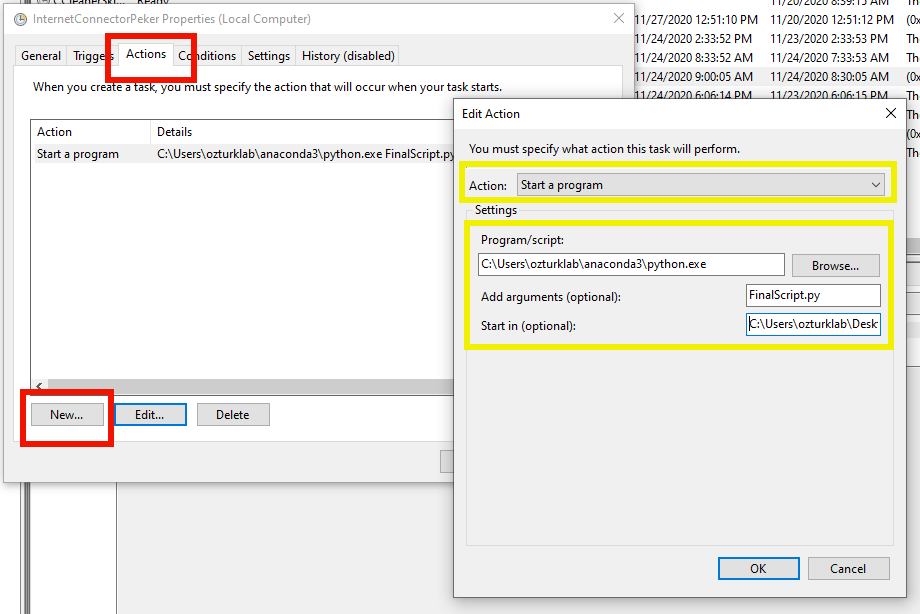
\includegraphics[angle=0,origin=c,width = .8\linewidth]{Section_Ethernet/Figures/TaskCreationAction.png}
		\caption{Script and arguments related fields under Triggers tab.}
		\label{fig:TaskAction}
	\end{figure}

 \item On the Conditions tab, as shown in Figure\ref{fig:TaskConditions}, most of 
 the fields are related with hardware such as whether you have a laptop which can
 run on battery or not. Therefore you can simply keep it as shown in Figure
 \ref{fig:TaskConditions}
	\begin{figure}[H]
		\centering
		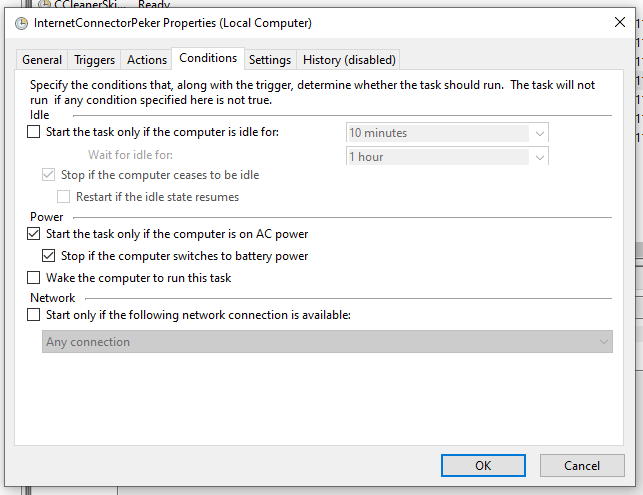
\includegraphics[angle=0,origin=c,width = .8\linewidth]{Section_Ethernet/Figures/TaskCreationConditions.png}
		\caption{Already prepared Conditions tab.}
		\label{fig:TaskConditions}
	\end{figure}

 \item On the Setting tab, as shown in Figure\ref{fig:TaskSettings}, you can again
 set relevant fields as shown in Figure\ref{fig:TaskSettings}.
	\begin{figure}[H]
		\centering
		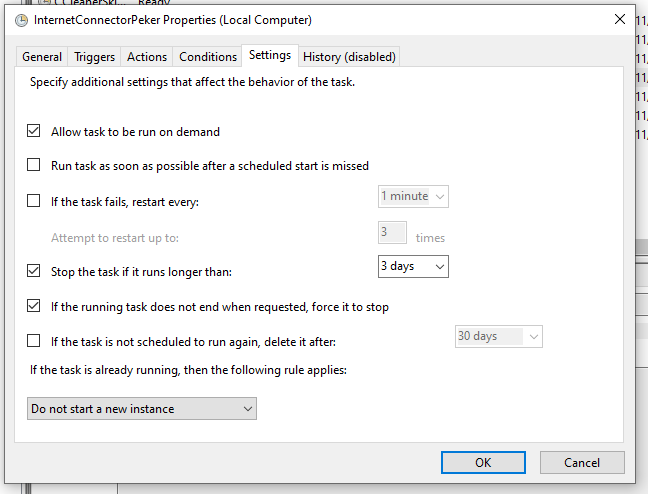
\includegraphics[angle=0,origin=c,width = .8\linewidth]{Section_Ethernet/Figures/TaskCreationSettings.png}
		\caption{Already prepared Settings tab.}
		\label{fig:TaskSettings}
	\end{figure}

 \item Once you are done with setting up your scheduled task, save it and close its
 window. This will add your new task to default windows tasks as shown in 
 Figure\ref{fig:TaskRun}. Right-click on your task and run it for the first time.
 After that point, it can run by itself.
	\begin{figure}[H]
		\centering
		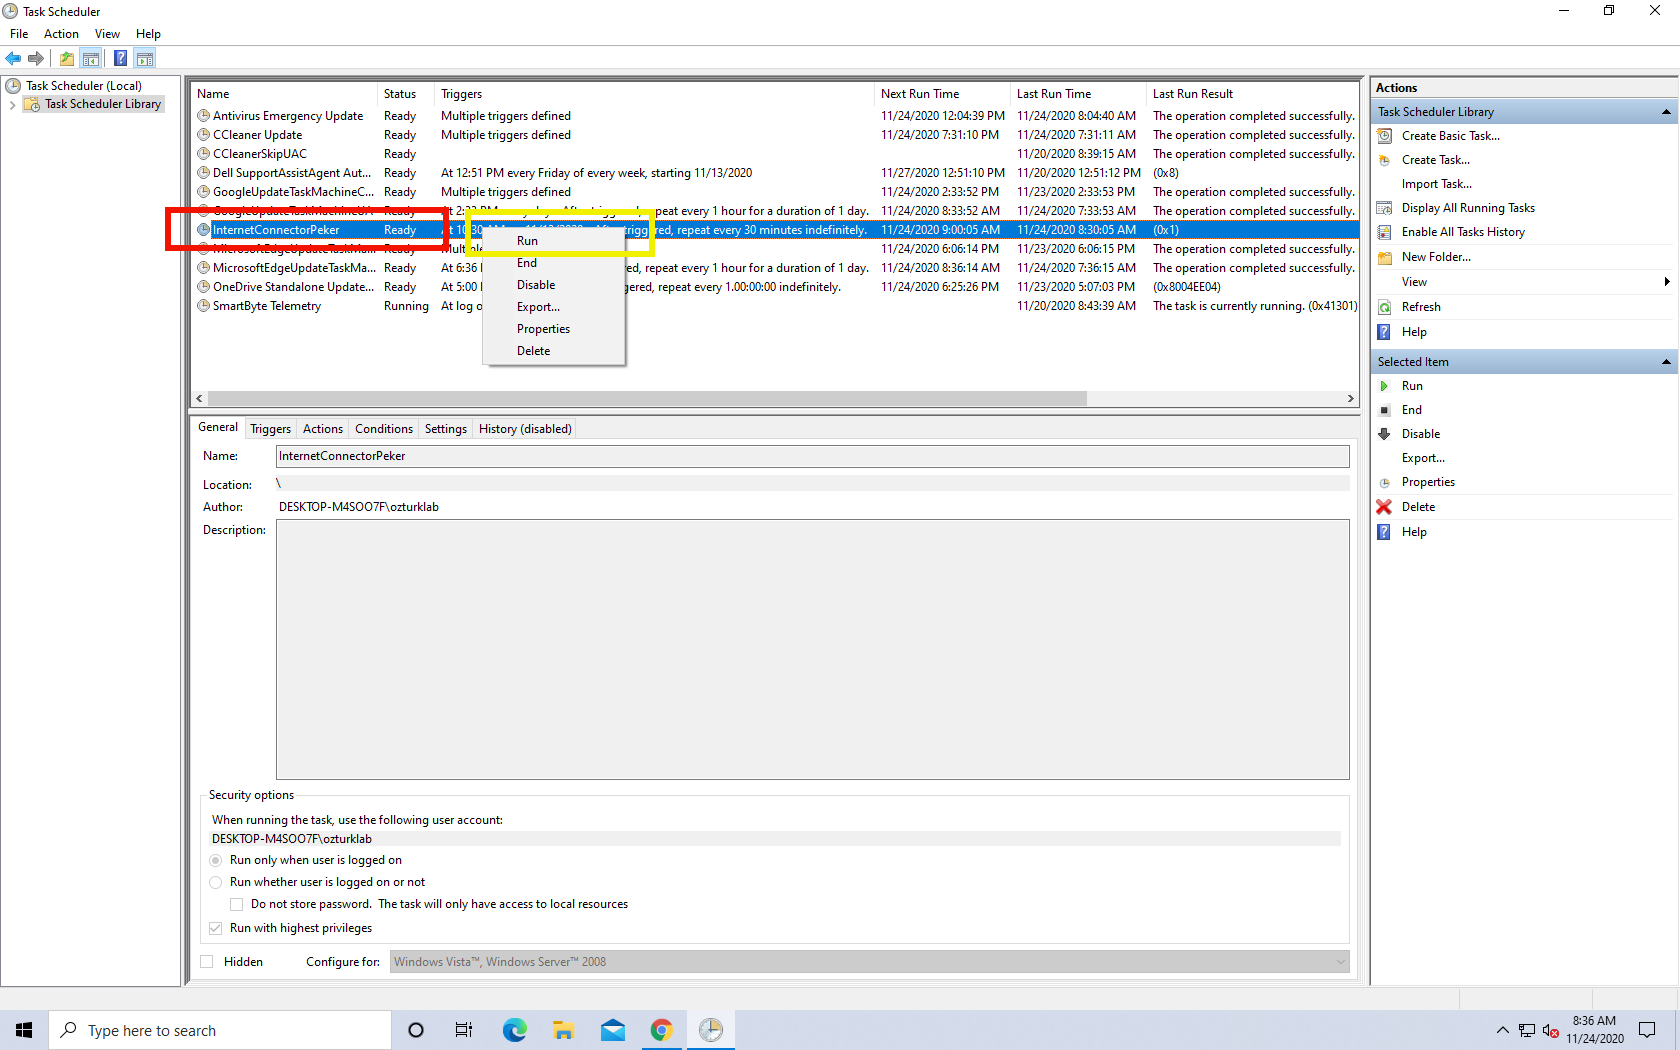
\includegraphics[angle=0,origin=c,width = .8\linewidth]{Section_Ethernet/Figures/TaskRun.png}
		\caption{First run of the new task.}
		\label{fig:TaskRun}
	\end{figure}
\end{enumerate}
